\documentclass[sigplan,screen]{acmart}

\settopmatter{printacmref=false}
\acmConference[ISSTA/SPLASH SRC'26]{ACM Student Research Competition}{October 2026}{Oakland, CA}
\fancyhead{}
\renewcommand\footnotetextcopyrightpermission[1]{}
\pagestyle{plain}

\usepackage{balance}
\usepackage{url}
\usepackage{tikz}
\usetikzlibrary{shapes.geometric, arrows.meta, positioning, fit}

\title{Template-Free Dynamic Invariant Detection}

\author{Erfan Arvan}
\affiliation{%
  \institution{New Jersey Institute of Technology}
  \city{Newark}
  \state{NJ}
  \country{USA}
}
\email{ea442@njit.edu}

\begin{abstract}
Dynamic invariant detectors such as Daikon infer likely program invariants
by evaluating candidate properties against execution traces.
However, Daikon's candidates are drawn from a fixed template library,
which prevents it from expressing properties that involve project-specific
logic or more than three variables.
We present \textsc{Oca}, a dynamic invariant detector that uses a large language
model (LLM) to propose candidates instead of deriving them from templates.
LLM-proposed invariants are more expressive, but their integration into
a dynamic analysis pipeline raises non-trivial research challenges
involving prompt design, context selection, and scalability.
We address these challenges and evaluate \textsc{Oca} on the Defects4J benchmark,
showing that it infers invariants beyond Daikon's expressive reach,
with ongoing evaluation of their bug-detection capability in property-based testing.
\end{abstract}

\begin{document}
\maketitle

\input{macros}

\section{Problem and Motivation}

Program invariants---properties that hold at every execution of a program
point---are foundational to testing, verification, and program understanding~\cite{ernst2007daikon}.
Dynamic invariant detectors such as Daikon~\cite{ernst2007daikon}
infer likely invariants automatically from execution traces,
avoiding the burden of manual specification.
Daikon is widely used in research and practice~\cite{pei2023llm,sun2025classinvgen},
but its design imposes a hard expressive ceiling:
it generates candidates from a fixed template library,
so any invariant that cannot be expressed within that grammar
is never even considered.
Concretely, Daikon cannot express (1)~properties involving
project-specific methods or domain abstractions, or
(2)~relations among more than three variables.
These limitations matter in practice:
real programs frequently contain semantic constraints
that cut across these boundaries.
Adding new templates does not solve the problem: run-time cost scales with candidate count, so template libraries must remain small.

Recent work has begun to explore LLMs as a source of invariant candidates~\cite{endres2024llm,pei2023llm,cao2025clause2inv,ma2025specgen,sun2025classinvgen},
but prior efforts were manual, limited in scope, or restricted to specific invariant classes
and did not produce a validated, end-to-end tool for method-level pre- and post-conditions.
We fill this gap with \textsc{Oca}\footnote{Oca is a South American root vegetable, chosen as a nod to Daikon.}, a dynamic invariant detector
that replaces Daikon's template library with LLM-generated candidates.
Like Daikon, \textsc{Oca} validates candidates against program executions.
However, because \textsc{Oca}'s candidates are arbitrary expressions,
storing the full program state needed to check them offline is not feasible;
instead, \textsc{Oca} injects candidates into the program source as guarded run-time checks
and validates them by executing the program's existing test suite.
Only executed candidates that are never falsified are reported as held.

\section{Research Challenges}

Substituting an LLM for a template library is not straightforward.
We identify five challenges that any such system must address.
The challenges fall into two groups.
The first concerns eliciting useful output from the LLM:
without careful choices of prompt design and context,
models produce vacuous or irrelevant candidates (C1, C2).
The second, and more fundamental, concerns the fact that LLM-generated invariants
can be poorly behaved in ways that manually-chosen templates never are---they
may be syntactically invalid, have side effects that corrupt program state,
or cause non-termination (C3, C4, C5).

\paragraph{C1: Designing prompts that elicit well-formed invariants.}
Without careful prompt design, an LLM may produce vacuous,
trivially true, or ill-structured properties.
The space of possible prompting strategies is large,
and the best strategy for invariant generation is not known in advance.

\paragraph{C2: Providing effective context.}
LLMs are sensitive to the context supplied in their prompts.
Too little context yields trivial or irrelevant invariants;
too much wastes token budget and can distract the model.
The right granularity is not obvious and cannot be determined a priori.

\paragraph{C3: Handling syntactically invalid candidates.}
LLM-generated expressions are not guaranteed to be syntactically valid Java.
They may reference out-of-scope identifiers, violate typing constraints,
or fail to compile when inserted into the program.
Even candidates that compile may cause test failures at run time.

\paragraph{C4: Ensuring invariant evaluation is side-effect free.}
Evaluating an LLM-generated invariant may cause side effects, such as calling a method that modifies program state,
corrupting the state that subsequent invariants are evaluated against
and causing valid invariants to be falsified.
A subtler instance arises when a called method has injected invariants:
those guards execute against inputs that exist only because an invariant
is being evaluated, and may be falsified incorrectly as a result.

\paragraph{C5: Handling suspected non-terminating candidates.}
LLM-generated invariants may cause non-termination during evaluation.

\section{Approach: \textsc{Oca}}

Figure~\ref{fig:pipeline} shows the \textsc{Oca} pipeline.
\textsc{Oca} begins by copying the target project into an isolated working directory
and scanning the source tree with JavaParser to identify method entry and exit points as program points.

\begin{figure}[t]
\centering
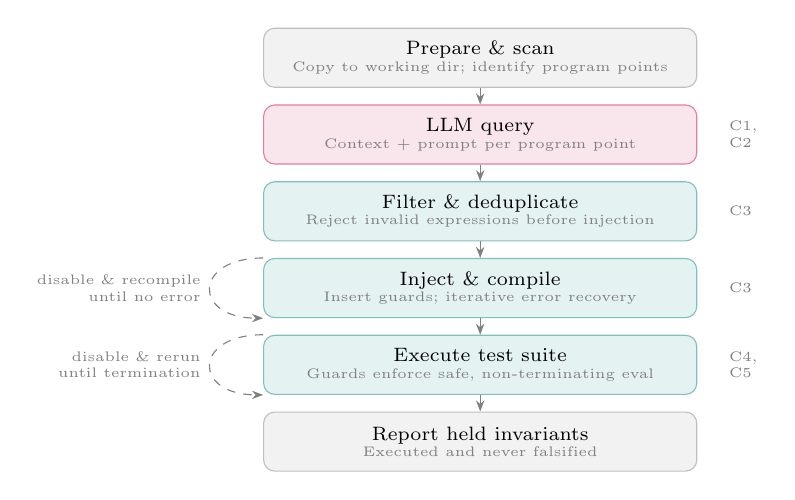
\begin{tikzpicture}[
  node distance=6pt,
  box/.style={rectangle, rounded corners=4pt, draw, minimum width=5.5cm, minimum height=0.75cm, align=center, font=\scriptsize},
  purplebox/.style={box, fill=purple!10, draw=purple!50},
  tealbox/.style={box, fill=teal!10, draw=teal!50},
  graybox/.style={box, fill=gray!10, draw=gray!50},
  clabel/.style={font=\tiny, text=gray},
  arr/.style={-{Stealth[length=4pt]}, gray},
  darr/.style={-{Stealth[length=4pt]}, gray, dashed},
]
\node[graybox] (scan)    {Prepare \& scan\\[-2pt]{\tiny\color{gray}Copy to working dir; identify program points}};
\node[purplebox, below=of scan]   (llm)     {LLM query\\[-2pt]{\tiny\color{gray}Context + prompt per program point}};
\node[tealbox, below=of llm]      (filter)  {Filter \& deduplicate\\[-2pt]{\tiny\color{gray}Reject invalid expressions before injection}};
\node[tealbox, below=of filter]   (inject)  {Inject \& compile\\[-2pt]{\tiny\color{gray}Insert guards; iterative error recovery}};
\node[tealbox, below=of inject]   (exec)    {Execute test suite\\[-2pt]{\tiny\color{gray}Guards enforce safe, non-terminating eval}};
\node[graybox, below=of exec]     (report)  {Report held invariants\\[-2pt]{\tiny\color{gray}Executed and never falsified}};

\draw[arr] (scan)   -- (llm);
\draw[arr] (llm)    -- (filter);
\draw[arr] (filter) -- (inject);
\draw[arr] (inject) -- (exec);
\draw[arr] (exec)   -- (report);

\draw[darr] (inject.north west) to[out=180,in=180,looseness=3] node[midway, clabel, left, align=right]{disable \& recompile\\until no error} (inject.south west);
\draw[darr] (exec.north west)   to[out=180,in=180,looseness=3] node[midway, clabel, left, align=right]{disable \& rerun\\until termination} (exec.south west);

\node[clabel, right=8pt of llm, align=left]    {C1,\\C2};
\node[clabel, right=8pt of filter] {C3};
\node[clabel, right=8pt of inject] {C3};
\node[clabel, right=8pt of exec, align=left]   {C4,\\C5};
\end{tikzpicture}
\caption{The \textsc{Oca} pipeline. Each stage addresses one or more research challenges (C1--C5).}
\label{fig:pipeline}
\end{figure}

For each program point, \textsc{Oca} queries an LLM with a prompt constructed
from a configurable set of typed context dimensions extracted statically from the source.
To address C1, we evaluated six prompting strategies---baseline direct prompting,
few-shot examples, chain-of-thought, stepwise decomposition, self-refinement,
and multi-sample agreement---on Apache Hudi~\cite{hudi}, libGDX~\cite{libgdx}, and RxJava~\cite{rxjava};
few-shot prompting produced the most held invariants and was selected as the default.
To address C2, we conducted an open-coding analysis of 187 recent LLM-based SE papers
from top venues to derive a taxonomy of context strategies,
then evaluated each on the same three projects
to select the configuration that maximizes held invariants.
Generated candidates are filtered and deduplicated,
then injected into the working copy as guarded run-time checks
and compiled iteratively; invalid candidates that survive filtering
are disabled until compilation succeeds (C3).
During execution, guards suppress nested evaluation
when another check is already active on the same thread (C4),
and a background monitor detects and disables suspected non-terminating candidates
at the per-invariant level without discarding results for others (C5).
Invariants that compile, execute at least once, and are never falsified are reported as held.

\section{Preliminary Results}

Table~\ref{tab:expr} shows preliminary expressiveness results
across twelve Defects4J~\cite{just2014defects4j} projects
using fixed program versions to avoid confounding with bug-induced behavior.
These results were obtained using a fixed baseline context configuration;
the empirically selected configuration from C2 is currently being evaluated.
We define an invariant as \emph{expressive} if it involves project-specific method calls
(criterion Daikon cannot satisfy by design)
or relates more than three variables
(a hard structural limit in Daikon's template grammar).

\begin{table}[h]
\centering
\caption{Expressiveness of \textsc{Oca}-inferred invariants across Defects4J.
\#Inv = total held invariants; Var$>$3 = invariants with $>$3 variables;
PSPM = invariants with project-specific method calls.}
\label{tab:expr}
\footnotesize
\begin{tabular*}{\columnwidth}{@{\extracolsep{\fill}}lrrr@{}}
\hline
\textbf{Project} & \textbf{\#Inv} & \textbf{Var$>$3 (\%)} & \textbf{PSPM (\%)} \\
\hline
Cli       &   963 &  1.0 &  9.0 \\
Closure   &  2117 &  1.1 & 28.3 \\
Codec     &  1869 &  2.0 & 23.1 \\
Compress  &  1546 &  0.7 & 10.0 \\
Csv       &   469 &  0.6 &  9.6 \\
Gson      &  1635 &  2.0 & 10.4 \\
JacksonDB &  1185 &  1.0 & 11.7 \\
Jsoup     &  1677 &  0.8 & 19.8 \\
Lang      &  3382 &  6.7 & 24.7 \\
Math      &  3518 &  2.5 &  7.7 \\
Mockito   &  1610 &  1.2 & 21.3 \\
Time      &  1007 &  1.7 & 17.4 \\
\hline
\textbf{Avg} & & \textbf{1.8} & \textbf{16.1} \\
\hline
\end{tabular*}
\end{table}

Across projects, an average of 16\% of held invariants involve project-specific logic
and 1.8\% relate more than three variables---both categories
entirely outside Daikon's expressive reach.
These are conservative figures: they exclude other forms of semantic richness
(e.g., nested logical structure) that also exceed Daikon's grammar.

Ongoing evaluation on buggy Defects4J versions measures whether these invariants improve bug detection in property-based testing relative to Daikon.

\section{Contributions}

This work makes the following contributions:

\begin{itemize}
  \item A characterization of the research challenges in integrating LLMs
        into a dynamic invariant detection pipeline (C1--C5).
  \item A systematic study of prompt and context strategies for LLM-based invariant generation.
  \item \textsc{Oca}, an end-to-end tool that addresses these challenges
        for Java programs, supporting both cloud-hosted and locally hosted LLMs.
  \item An empirical evaluation on Defects4J showing that \textsc{Oca}
        infers invariants beyond Daikon's expressive reach,
        with ongoing evaluation of downstream bug detection.
\end{itemize}

\begin{acks}
I thank Martin Kellogg and Michael D. Ernst for advising this research.
\end{acks}

\balance

\bibliographystyle{ACM-Reference-Format}
\begin{thebibliography}{3}

\bibitem{hudi}
Apache Software Foundation.
Apache Hudi.
\url{https://github.com/apache/hudi}, 2024.

\bibitem{libgdx}
libGDX Contributors.
libGDX.
\url{https://github.com/libgdx/libgdx}, 2024.

\bibitem{rxjava}
ReactiveX Contributors.
RxJava.
\url{https://github.com/ReactiveX/RxJava}, 2024.

\bibitem{just2014defects4j}
R.~Just, D.~Jalali, and M.~D. Ernst.
Defects4J: A database of existing faults to enable controlled testing studies for Java programs.
In \emph{Proc. Intl. Symp. on Software Testing and Analysis (ISSTA)}, pp. 437--447, 2014.

\bibitem{ernst2007daikon}
M.~D. Ernst, J.~H. Perkins, P.~J. Guo, S.~McCamant, C.~Pacheco,
M.~S. Tschantz, and C.~Xiao.
The Daikon system for dynamic detection of likely invariants.
\emph{Science of Computer Programming}, 69(1--3):35--45, 2007.

\bibitem{endres2024llm}
M.~Endres, S.~Fakhoury, S.~Chakraborty, and S.~K. Lahiri.
Can large language models transform natural language intent into formal method postconditions?
\emph{Proc. ACM Softw. Eng.}, 1(FSE):1889--1912, 2024.

\bibitem{sun2025classinvgen}
C.~Sun et al.
ClassInvGen: Class invariant synthesis using large language models.
In \emph{Intl. Symp. on AI Verification}, pp. 64--96, 2025.

\bibitem{pei2023llm}
K.~Pei, D.~Bieber, K.~Shi, C.~Sutton, and P.~Yin.
Can large language models reason about program invariants?
In \emph{International Conference on Machine Learning}, pp. 27496--27520, 2023.

\bibitem{cao2025clause2inv}
W.~Cao, G.~Wu, T.~Xu, Y.~Yao, H.~Wei, T.~Chen, and X.~Ma.
Clause2Inv: A generate-combine-check framework for loop invariant inference.
\emph{Proc. ACM Softw. Eng.}, 2(ISSTA):1009--1030, 2025.

\bibitem{ma2025specgen}
L.~Ma, S.~Liu, Y.~Li, X.~Xie, and L.~Bu.
SpecGen: Automated generation of formal program specifications via large language models.
In \emph{Proc. 47th Intl. Conf. on Software Engineering (ICSE)}, pp. 666, 2025.

\end{thebibliography}

\end{document}
